\documentclass[spanish,a4paper,11pt,twoside]{report}

%%%%%%%%%%%%%%%%%%%%%%%%%%%%%%%%%%%%%%%%%%%%%%%%%%%%%%%%%%%%%%%%%%%%%%%%%%%%%%%
\usepackage[dvips]{graphicx}
\usepackage[dvips]{epsfig}
\usepackage[latin1]{inputenc}
\usepackage[spanish]{babel}
\usepackage{alltt}
\usepackage{templates/algorithm}
\usepackage{templates/algorithmic}
\usepackage{templates/multirow}

%%%%%%%%%%%%%%%%%%%%%%%%%%%%%%%%%%%%%%%%%%%%%%%%%%%%%%%%%%%%%%%%%%%%%%%%%%%%%%%

\newcommand{\SONY}{{\sc Sony}}
\newcommand{\MICROSOFT}{{\sc Microsoft}}
\newcommand{\GCC}{\textsf{\textsc{G}CC}}
\newcommand{\INTEL}{\textsf{\textsc{I}ntel}}

%%% Traducimos el pseudocodigo
\renewcommand{\algorithmicwhile}{\textbf{mientras}}
\renewcommand{\algorithmicend}{\textbf{fin}}
\renewcommand{\algorithmicdo}{\textbf{hacer}}
\renewcommand{\algorithmicif}{\textbf{si}}
\renewcommand{\algorithmicthen}{\textbf{entonces}}
\renewcommand{\algorithmicrepeat}{\textbf{repetir}}
\renewcommand{\algorithmicuntil}{\textbf{hasta que}}
\renewcommand{\algorithmicelse}{\textbf{en otro caso}}
\renewcommand{\algorithmicfor}{\textbf{para}}

%\newcommand{\RETURN}{\textbf{retornar} }
\newcommand{\RET}{\STATE \textbf{retornar} }
\newcommand{\TO}{\textbf{hasta} }
\newcommand{\AND}{\textbf{y} }
\newcommand{\OR}{\textbf{o} }

%%%%%%%%%%%%%%%%% Creamos un entorno para listar c�digo fuente %%%%%%%%%%%%%%%
\newenvironment{sourcecode}
{\begin{list}{}{\setlength{\leftmargin}{1em}}\item\scriptsize\bfseries}
{\end{list}}

\newenvironment{littlesourcecode}
{\begin{list}{}{\setlength{\leftmargin}{1em}}\item\tiny\bfseries}
{\end{list}}

\newenvironment{summary}
{\par\noindent\begin{center}\textbf{Abstract}\end{center}\begin{itshape}\par\noindent}
{\end{itshape}}

\newenvironment{keywords}
{\begin{list}{}{\setlength{\leftmargin}{1em}}\item[\hskip\labelsep \bfseries Keywords:]}
{\end{list}}

\newenvironment{palabrasClave}
{\begin{list}{}{\setlength{\leftmargin}{1em}}\item[\hskip\labelsep \bfseries Palabras clave:]}
{\end{list}}


%%%%%%%%%%%%%%%%%%%%%%%%%%%%%%%%%%%%%%%%%%%%%%%%%%%%%%%%%%%%%%%%%%%%%%%%%%%%%%%
% Format
%%%%%%%%%%%%%%%%%%%%%%%%%%%%%%%%%%%%%%%%%%%%%%%%%%%%%%%%%%%%%%%%%%%%%%%%%%%%%%%

%%\topmargin -4 mm
%\topmargin -21 mm
%\headheight 10 mm
%\headsep 10 mm

%\textheight 229 mm
%\textheight 246 mm

%\oddsidemargin -5.4 mm
%\evensidemargin -5.4 mm
\oddsidemargin 5 mm
\evensidemargin 5 mm

%\oddsidemargin -3 mm
%\evensidemargin -3 mm

%\textwidth 17 cm
\textwidth 15 cm
%\columnsep 10 mm

\input{amssym.def}

%%%%%%%%%%%%%%%%%%%%%%%%%%%%%%%%%%%%%%%%%%%%%%%%%%%%%%%%%%%%%%%%%%%%%%%%%%%%%%%

\begin{document}

%%%%%%%%%%%%%%%%%%%%%%%%%%%%%%%%%%%%%%%%%%%%%%%%%%%%%%%%%%%%%%%%%%%%%%%%%%%%%%%
% First Page 
%%%%%%%%%%%%%%%%%%%%%%%%%%%%%%%%%%%%%%%%%%%%%%%%%%%%%%%%%%%%%%%%%%%%%%%%%%%%%%%

\pagestyle{empty}
\thispagestyle{empty}


\newcommand{\HRule}{\rule{\linewidth}{1mm}}
\setlength{\parindent}{0mm}
\setlength{\parskip}{0mm}
\vspace*{\stretch{1}}

\begin{center}

\includegraphics[width=0.2\textwidth]{images/logotipo-secundario-ULL}\\[0.25cm]
\end{center}

\HRule
\begin{center}
        {\Huge T�tulo del trabajo} \\[2.5mm] 
        {\Huge Subt�tulo} \\[2.5mm]
        {\Large Autor (o autores)} \\[5mm]
        {\Large \textit{Grupo ($1\mid2$) }} \\[5mm]


        {\em T�cnicas Experimentales. $1^{er}$ curso. $2^{do}$ semestre} \\[5mm]
        Lenguajes y Sistemas Inform�ticos \\[5mm]
        Facultad de Matem�ticas \\[5mm]
        
        Universidad de La Laguna \\
\end{center}
\HRule
\vspace*{\stretch{2}}
\begin{center}
  La Laguna, \today 
\end{center}

%%%%%%%%%%%%%%%%%%%%%%%%%%%%%%%%%%%%%%%%%%%%%%%%%%%%%%%%%%%%%%%%%%%%%%%%%%%%%%%

%%%%%%%%%%%%%%%%%%%%%%%%%%%%%%%%%%%%%%%%%%%%%%%%%%%%%%%%%%%%%%%%%%%%%%%%%%%%%%%
\newpage{\pagestyle{empty}\cleardoublepage}

\pagestyle{myheadings} %my head defined by markboth or markright
% No funciona bien \markboth sin "twoside" en \documentclass, pero al
% ponerlo se dan un mont�n de errores de underfull \vbox, con lo que no se
% ha puesto.
\markboth{Nombre del alumno}{T�tulo del trabajo}

%%%%%%%%%%%%%%%%%%%%%%%%%%%%%%%%%%%%%%%%%%%%%%%%%%%%%%%%%%%%%%%%%%%%%%%%%%%%%%%
%Numeracion en romanos
\renewcommand{\thepage}{\roman{page}}
\setcounter{page}{1}

%%%%%%%%%%%%%%%%%%%%%%%%%%%%%%%%%%%%%%%%%%%%%%%%%%%%%%%%%%%%%%%%%%%%%%%%%%%%%%%

\tableofcontents

%%%%%%%%%%%%%%%%%%%%%%%%%%%%%%%%%%%%%%%%%%%%%%%%%%%%%%%%%%%%%%%%%%%%%%%%%%%%%%%
\newpage{\pagestyle{empty}\cleardoublepage}

\listoffigures

%%%%%%%%%%%%%%%%%%%%%%%%%%%%%%%%%%%%%%%%%%%%%%%%%%%%%%%%%%%%%%%%%%%%%%%%%%%%%%%
\newpage{\pagestyle{empty}\cleardoublepage}

\listoftables

%%%%%%%%%%%%%%%%%%%%%%%%%%%%%%%%%%%%%%%%%%%%%%%%%%%%%%%%%%%%%%%%%%%%%%%%%%%%%%%
\newpage{\pagestyle{empty}\cleardoublepage}

%%%%%%%%%%%%%%%%%%%%%%%%%%%%%%%%%%%%%%%%%%%%%%%%%%%%%%%%%%%%%%%%%%%%%%%%%%%%%%%
%Numeracion a partir del capitulo I
\renewcommand{\thepage}{\arabic{page}}
\setcounter{page}{1}

\setlength{\parindent}{5mm}

%%%%%%%%%%%%%%%%%%%%%%%%%%%%%%%%%%%%%%%%%%%%%%%%%%%%%%%%%%%%%%%%%%%%%%%%%%%%%%%
\chapter{Motivaci�n y objetivos}
\label{chapter:obj}

%%%%%%%%%%%%%%%%%%%%%%%%%%%%%%%%%%%%%%%%%%%%%%%%%%%%%%%%%%%%%%%%%%%%%%%%%%%%%
% Chapter 1: Motivaci�n y Objetivos 
%%%%%%%%%%%%%%%%%%%%%%%%%%%%%%%%%%%%%%%%%%%%%%%%%%%%%%%%%%%%%%%%%%%%%%%%%%%%%%%


Para comenzar este trabajo, expondremos a continuaci�n los fines de la realizaci�n de este proyecto
que implica la resoluci�n de un problema con la utilizaci�n de un lenguaje de programaci�n interpretado.  

%---------------------------------------------------------------------------------
  \section{Objetivo principal}
\label{1:sec:1}
  La intenci�n principal para el desarrollo de este informe es el planteamiento de un experimento cuyo fin 
es el c�lculo del �rea de una funci�n dada de la forma m�s precisa posible. 
En este desarrollo interviene un m�todo de integraci�n num�rica, lo que conlleva no s�lo un aprendizaje en el �mbito inform�tico 
(referido a la utilizaci�n de algoritmos y sentencias l�gicas) sino que adem�s permite hacer un enfoque matem�tico 
que obliga a alcanzar una mayor destreza en �nalisis matem�tico\footnote{Es una rama de la ciencia matem�tica que se empieza a desarrollar a partir
 del inicio de la formulaci�n del c�lculo y estudia conceptos como la continuidad, la integraci�n y la diferenciabilidad de diversas formas}.

%---------------------------------------------------------------------------------
\section{Secci�n Dos}
\label{1:sec:2}
  Primer p�rrafo de la segunda secci�n.

\begin{itemize}
  \item Item 1
  \item Item 2
  \item Item 3
\end{itemize}



%%%%%%%%%%%%%%%%%%%%%%%%%%%%%%%%%%%%%%%%%%%%%%%%%%%%%%%%%%%%%%%%%%%%%%%%%%%%%%%
\chapter{Fundamentos te�ricos}
\label{chapter:teo}

%%%%%%%%%%%%%%%%%%%%%%%%%%%%%%%%%%%%%%%%%%%%%%%%%%%%%%%%%%%%%%%%%%%%%%%%%%%%%%%
% Chapter 2: Fundamentos Te�ricos 
%%%%%%%%%%%%%%%%%%%%%%%%%%%%%%%%%%%%%%%%%%%%%%%%%%%%%%%%%%%%%%%%%%%%%%%%%%%%%%%

%++++++++++++++++++++++++++++++++++++++++++++++++++++++++++++++++++++++++++++++

En este cap�tulo se han de presentar los antecedentes te�ricos y pr�cticos que
apoyan el tema objeto de la investigaci�n.

%++++++++++++++++++++++++++++++++++++++++++++++++++++++++++++++++++++++++++++++

\section{Primer apartado del segundo cap�tulo}
\label{2:sec:1}
  Primer p�rrafo de la primera secci�n.

\section{Segundo apartado del segundo cap�tulo}
\label{2:sec:2}
La f�rmula simple se define como:
\[\int_{a}^{b} f(x)\text{d}x ~ \frac{b-a}{6}\big[f(a)+4f(m)+f(b)\big]\]\par
 
Por otra parte, la f�rmula compuesta aparece como:

\[\int_{a}^{b} f(x)\text{d}x ~ \frac{h}{3}\big[f(x_0)+2\sum_{j=1}{\frac{n}{2-1}} f(x_{2j})+4 \sum_{j=1}{\frac{n}{2}}f(x_{2j-1})+f(x_n)\]


En nuestro proyecto, se nos ha propuesto utilizar principalmente el intervalo [-1,1] pero debido al tipo de experimento que deseamos 
realizar, adem�s de �ste, otros intervalos de diferentes tama�os para que nos produzcan resultados variados y se determine, como se ha expuesto aqu�,
la considerable diferencia entre la utilizaci�n de cada una de las f�rmulas y la variaci�n entre las diferentes cotas.




%%%%%%%%%%%%%%%%%%%%%%%%%%%%%%%%%%%%%%%%%%%%%%%%%%%%%%%%%%%%%%%%%%%%%%%%%%%%%%%
\chapter{Procedimiento experimental}
\label{chapter:exp}

%%%%%%%%%%%%%%%%%%%%%%%%%%%%%%%%%%%%%%%%%%%%%%%%%%%%%%%%%%%%%%%%%%%%%%%%%%%%%%%
% Chapter 3: Procedimiento experimental 
%%%%%%%%%%%%%%%%%%%%%%%%%%%%%%%%%%%%%%%%%%%%%%%%%%%%%%%%%%%%%%%%%%%%%%%%%%%%%%%

Este cap�tulo ha de contar con seccciones para la descripci�n de los experimentos 
y del material.
%
Tambi�n debe haber una secci�n para los resultados obtenidos y una �ltima de 
an�lisis de los resultados.

%++++++++++++++++++++++++++++++++++++++++++++++++++++++++++++++++++++++++++++++
\section{Descripci�n de los experimentos}
\label{3:sec:1}
Como se ha explicado en el cap�tulo dos, el m�todo propuesto tiene tanto f�rmula simple (para intervalos peque�os) como compuesta (para intervalos mayores).
Por ello, el experimento se basar� en la comparaci�n entre las f�rmulas, en el que se realizar�n pruebas de tiempo de ejecuci�n de ambas con 
diferentes intervalos,adem�s de distintas reiteraciones en el caso de la compuesta.
Por lo tanto se puede dividir en dos partes.
\subsection{Experimento con la f�rmula simple}
Esta parte del experimento comienza con la creaci�n de un m�dulo principal que contiene una definici�n de la funci�n y llamadas al usuario
con la intenci�n de que introduzca los intervalos deseados. Los resultados que se obtienen se guardar�n en un fichero que se pedir� tambi�n por teclado, 
pudiendo guardar variar ejecuciones en el mismo, es decir, sin que se sobrescriba al usar el mismo nombre.
En un m�dulo aparte, se calcular� el tiempo que tarda en ejecutarse cada intervalo y el tiempo que mantiene el cpu.
\subsection{Experimento con la f�rmula compuesta}
En cuanto a la segunda parte, se podr�a decir, que es una ampliaci�n de la primera. Dado que la f�rmula compuesta permite realizar el experimento con 
n�meros de reiteraciones diferentes se proponen dos programas en los que el n�mero de reiteraciones est� ya asignado, siendo 2 y 4 el n�mero de 
repeticiones que se har�n. Los intervalos de cuyos resultados se encuentran a continuaci�n, han sido de [-1,1],[-1,4],[2,8].
Al igual que en la primera parte se ver�n los tiempos trancurridos y los del CPU.
%++++++++++++++++++++++++++++++++++++++++++++++++++++++++++++++++++++++++++++++
\section{Descripci�n del material}
\label{3:sec:2}
\begin{itemize}
\item Para la realizaci�n de este trabajo, se ha utilizado la computadora, 
como herramienta principal. �sta posee una serie de recursos a la hora de trabajar , ya sea, programas, editores de texto(kate, vi...), consola, entre otros,
los cuales han sido �tiles, y empleados en este caso para la realizaci�n de este proyecto. A continuaci�n, daremos la informaci�n 
sobre el hadware, sistema operativo y compilador de la computadora utilizada para la realizaci�n de dicho trabajo:\par
Tipo de CPU: Pentium(R) Dual-Core  CPU      E5200  @ 2.50GHz \par
cache size: 2048 KB \par
CPU speed: 1200.000 Hz \par
vendor ID: GenuineIntel \par
Linux version: Linux-3.2.0-40-generic-i686-with-Ubuntu-12.04-precise \par
Python version: 2.7.3 \par
\item Adem�s, como hemos utilizado para la realizaci�n del informe,el ~\LaTeX, sistema de composici�n de textos orientado especialmente para la creaci�n de libros, documentos cient�ficos y t�cnicos
que contengan varias f�rmulas matem�ticas.   
  \item Para la presentaci�n con transparencias, empleamos un macro de ~\TeX, Beamer, ideado para realizar presentaci�n que permitan la inclusi�n de f�rmulas matem�ticas.
  \item Y por �ltimo, manejamos Python, que es un lenguaje de programaci�n interpretado. Sus ventajas son la rapid�z de desarrollo, debido a que no es necesario 
compilarlo, dicho lenguaje es multiplataforma y de codigo abierto.

\end{itemize}
%++++++++++++++++++++++++++++++++++++++++++++++++++++++++++++++++++++++++++++++
\section{Resultados obtenidos}
\label{3:sec:3}

A continuaci�n, se pueden ver las tablas y gr�ficas de los resultados que se han obtenido despu�s de realizar los experimentos:
\ref{fig:1}
\ref{fig:2}
\ref{fig:3}
\ref{tab:1}
\ref{tab:2}
\ref{tab:3}

%------------------------------------------------------------------------------

%------------------------------------------------------------------------------


%++++++++++++++++++++++++++++++++++++++++++++++++++++++++++++++++++++++++++++++
\section{An�lisis de los resultados}
\label{3:sec:4}
Como se ha visto en el apartado anterior, se han mostrado cuatro tablas en las que se representan los datos obtenidos, apareciendo en las dos primeras el �rea 
de la f�rmula simple, y en las segundas el tiempo transcurrido y el que ha tardado la CPU.
Centr�ndonos ahora en el an�lisis de los resultados que hemos obtenido en las gr�ficas, podemos decir que con los intervalos [-1,1] y [2,8] las resctas que 
se forman est�n m�s alejadas entre s� que en el intervalo que podr�amos considerar ni grande ni peque�o. Con esto, quedar�a probado lo explicado anteriormente, 
los fundamentos te�ricos, debido a que, como recordamos, la f�rmula simple se usa para intervalos peque�os y la compuesta para intervalos mayores.
Por otra parte,  se ha experimentado con el tiempo transcurrido para el tratamiento del m�todo y con el de ejecuci�n de la CPU. Como sabemos, el tiempo 
transcurrido durante la ejecuci�n del programa var�a dependiendo de la computadora que se use, a�n as� podemos apreciar que es mayor al realizar la f�rmula 
compuesta ya que las reiteraciones hacen que el programa se retrase.
En cuanto al tiempo de la CPU, no var�a en absoluto en ninguno de los intervalos puesto que la respuesta de la CPU es inmediata. 

%------------------------------------------------------------------------------

%--------------------------------------------------------------------------
\begin{table}[!ht]
\begin{center}
\begin{tabular}{|c||c||c|} \hline 
  \textbf{Intervalo} & \textbf{Area}  \\ \hline \hline
[-1,1] &  0693236856881
\\
\hline
[-1,4] & 0.633179114507
\\
\hline

[2,8] & 0.0539969133913
\\
\hline
\hline

\end{tabular}
\end{center}
\caption{Resultados experimentales del calculo del area (formula simple)}
\label{tab:1}
\end{table}


 %--------------------------------------------------------------------------
\begin{table}[!ht]
\begin{center}
\begin{tabular}{|c||c||c|} \hline 
\textbf{Intervalo} & \textbf{Area con iteracion = 4}  \\ \hline \hline
[-1,1] &  0.5813286
\\
\hline
[-1,4] & 0.646540956
\\
\hline

[2,8] & 0.0278711396576
\\
\hline
\hline

\end{tabular}
\end{center}
\caption{Resultados experimentales del calculo del area (formula compuesta)}
\label{tab:2}
\end{table}

 %--------------------------------------------------------------------------
\begin{table}[!ht]
\begin{center}
\begin{tabular}{|c||c||c|} \hline 
\textbf{Intervalo} & \textbf{Tiempo transcurrido}  & \textbf{Tiempo CPU}\\ \hline \hline
[-1,1] &  1.096754 $\text{e}^{-0.5}$& 0.0
\\
\hline
[-1,4] & 1.2159347$\text{e}^{-0.5}$ & 0.0
\\
\hline

[2,8] & 1.096725 $\text{e}^{-0.5}$& 0.0
\\
\hline
\hline

\end{tabular}
\end{center}
\caption{Resultados experimentales de tiempo(formula simple)}
\label{tab:3}
\end{table}

 %--------------------------------------------------------------------------
\begin{table}[!ht]
\begin{center}
\begin{tabular}{|c||c||c|} \hline 
\textbf{Intervalo} & \textbf{Tiempo transcurrido}  & \textbf{Tiempo CPU}\\ \hline \hline
[-1,1] &  9.059906$\text{e}^{-0.5}$ & 0.0
\\
\hline
[-1,4] & 1.001358 $\text{e}^{-0.5}$& 0.0
\\
\hline

[2,8] & 7.867813 $\text{e}^{-0.6}$& 0.0
\\
\hline
\hline

\end{tabular}
\end{center}
\caption{Resultados experimentales de tiempo (formula compuesta)}
\label{tab:2}
\end{table}
%------------------------------------------------------------------------------
\begin{figure}[!th]
\begin{center}
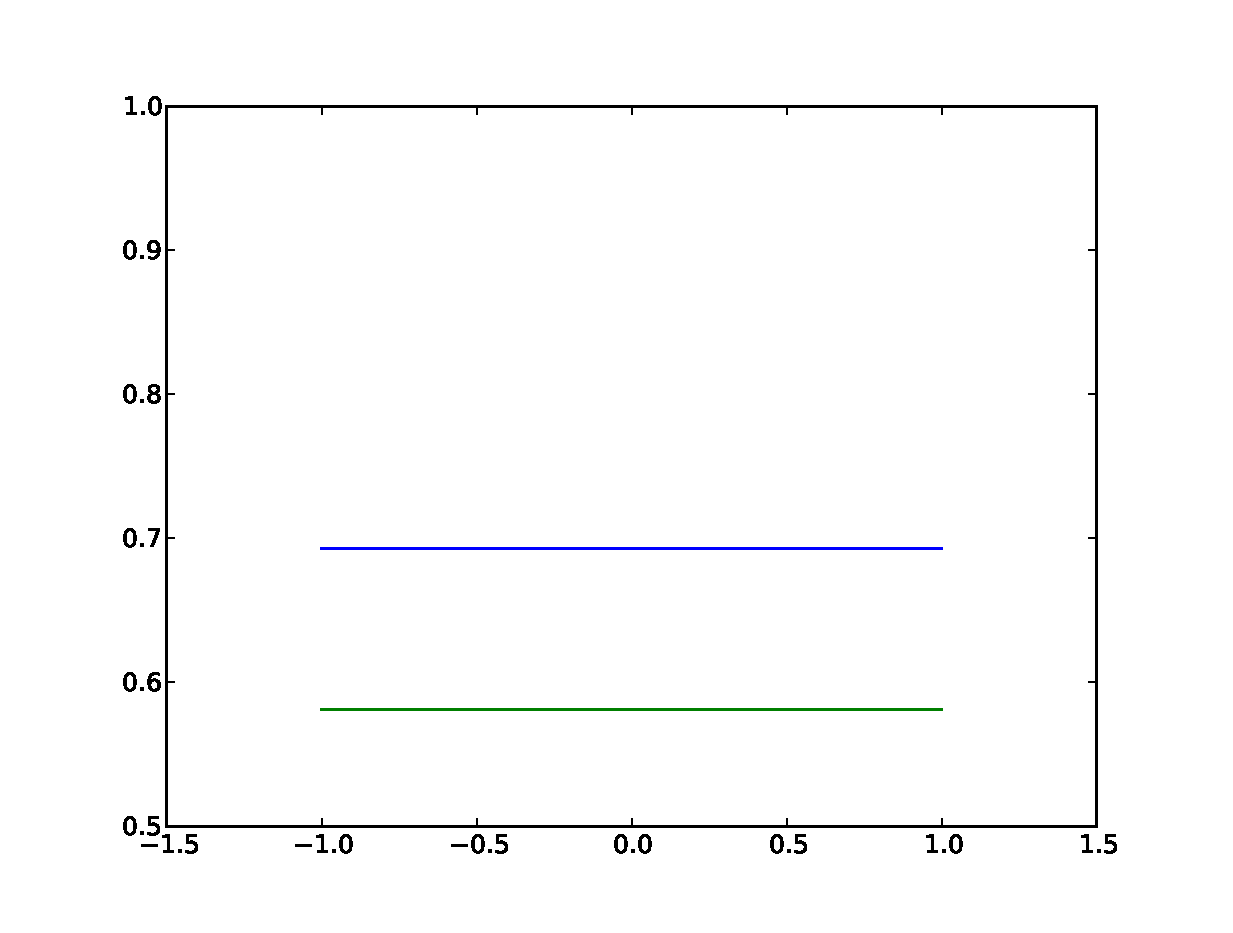
\includegraphics[width=0.75\textwidth]{images/1intervalo.eps}
\caption{Intervalo [-1,1]}
\label{fig:1}
\end{center}
\end{figure}

\begin{figure}[!th]
\begin{center}
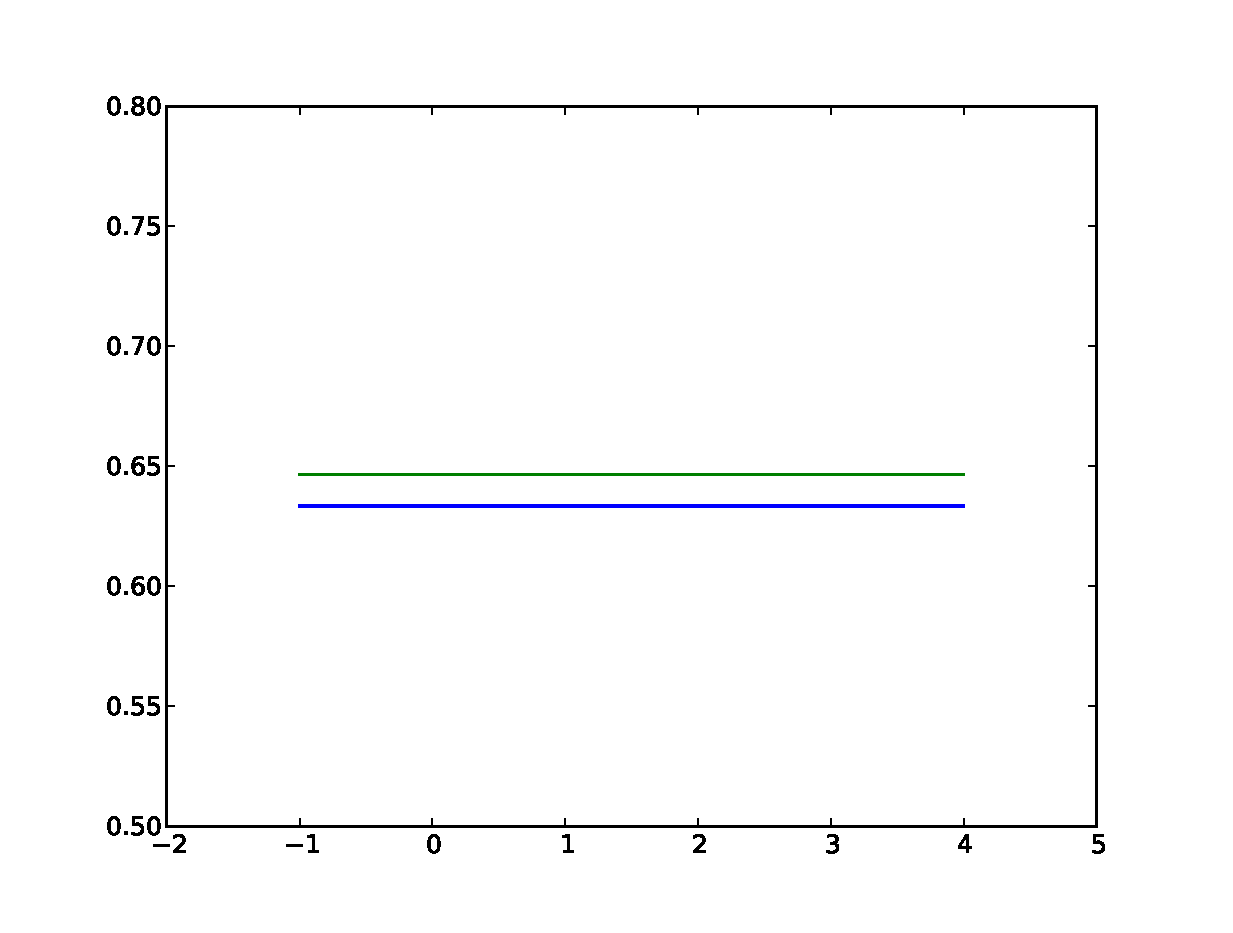
\includegraphics[width=0.75\textwidth]{images/2intervalo.eps}
\caption{Intervalo [-1,4]}
\label{fig:2}
\end{center}
\end{figure}
\begin{figure}[!th]
\begin{center}
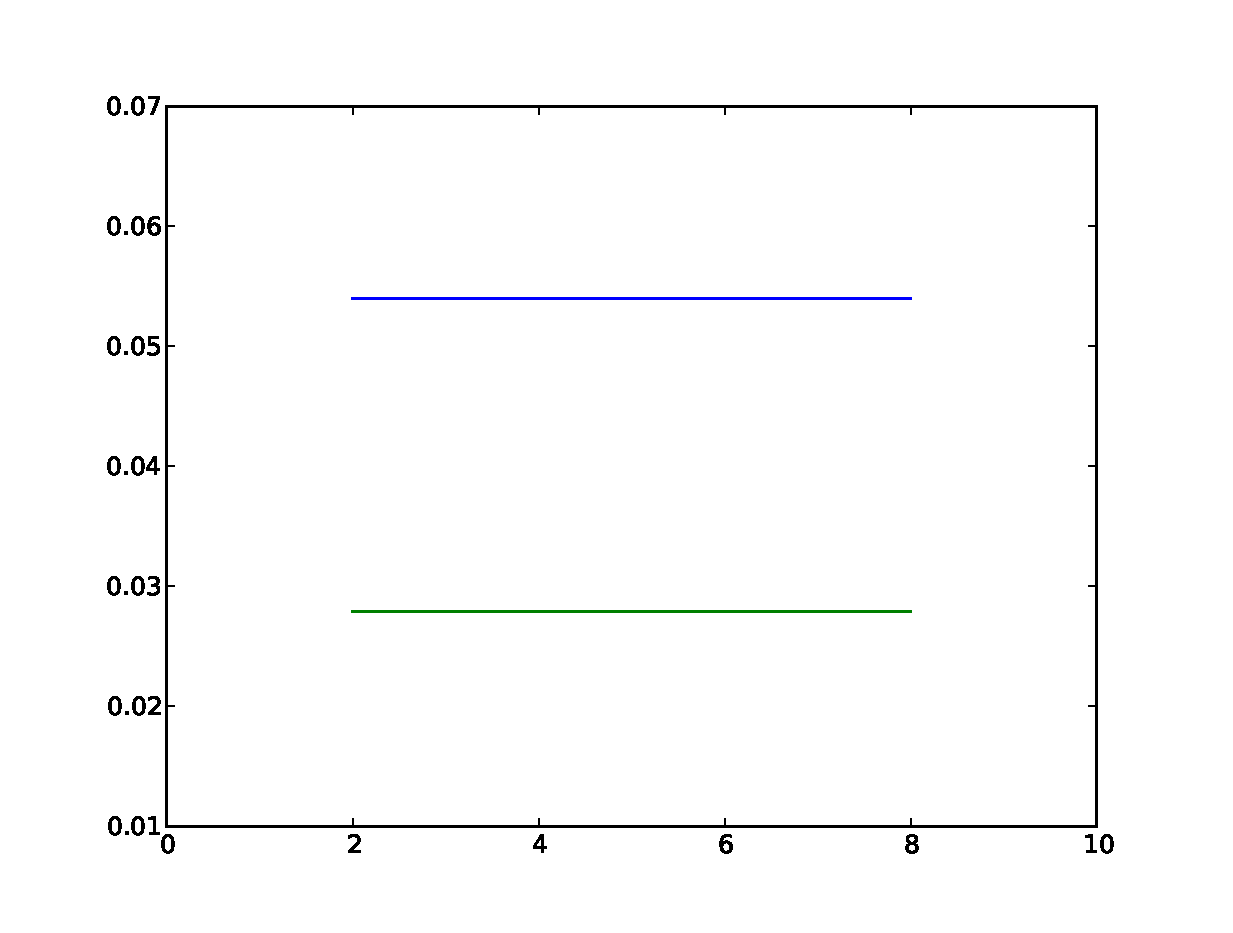
\includegraphics[width=0.75\textwidth]{images/3intervalo.eps}
\caption{Intervalo [2,8]}
\label{fig:3}
\end{center}
\end{figure}

%%%%%%%%%%%%%%%%%%%%%%%%%%%%%%%%%%%%%%%%%%%%%%%%%%%%%%%%%%%%%%%%%%%%%%%%%%%%%%%
\chapter{Conclusiones}
\label{chapter:conclusiones}

%%%%%%%%%%%%%%%%%%%%%%%%%%%%%%%%%%%%%%%%%%%%%%%%%%%%%%%%%%%%%%%%%%%%%%%%%%%%%
% Chapter 4: Conclusiones y Trabajos Futuros 
%%%%%%%%%%%%%%%%%%%%%%%%%%%%%%%%%%%%%%%%%%%%%%%%%%%%%%%%%%%%%%%%%%%%%%%%%%%%%%%
%No compila al escribir algunas de las tíldes
En este trabajo se presento el desarrollo de la resolucion del area de una funcion por el metodo de Simpson.
El objetivo ha sido la confeccion de un informe redactado en codigo ~\LaTeX, y unas transparecias en Beamer con este mismo lenguaje. 
Cabe decir, que el lenguaje de programacion con el que se ha confeccionado el experimento ha sido el python.
Se podría decir que la primera conclusion que hemos obtenido ha sido la verificacion de que los intervalos menores se usan para la formula simple y 
que los mayores para la formula compuesta.
Tambien, hemos visto que en los programas en los que intervienen definiciones de funciones no muy complejas el tiempo de la CPU es minimo.
A parte de esto, se puede concluir diciendo que hemos obtenido facilidades a la hora de creacion de codigos para resolucion de problemas, ademas de haber 
logrado aumentar las capacidades que ya se tenian con ~\LaTeX

%%%%%%%%%%%%%%%%%%%%%%%%%%%%%%%%%%%%%%%%%%%%%%%%%%%%%%%%%%%%%%%%%%%%%%%%%%%%%%%

%%%%%%%%%%%%%%%%%%%%%%%%%%%%%%%%%%%%%%%%%%%%%%%%%%%%%%%%%%%%%%%%%%%%%%%%%%%%%%%
\newpage{\pagestyle{empty}\cleardoublepage}
\thispagestyle{empty}
\begin{appendix}

\chapter{T�tulo del Ap�ndice 1}
\label{appendix:1}


\label{Apendice1:XXX}

\section{Formula simple }
\begin{center}
\begin{footnotesize}
\begin{verbatim}
 Nombre del fichero:
  modulo_simpson.py

 Autoras de dicho fichero:
   Nadia Chinea Chinea 
   Tania Gutierrez Gutierrez 
   Melanie Hernandez Alonso
  
 #!/usr/bin/python

import random, sys
from math import *

def f(x):
  return 1.0/(sqrt(2.0*pi))*exp((-x**2.0)/2)
  
def simpson(a,b):
  
  f1=(b-a)/6.0
  f2=f(a)+(4.0*f((a+b)/2.0))+f(b)
  
  return f1*f2   
  
if __name__ == '__main__':
  
  if (len(sys.argv)) == 4:
    a=float(sys.argv[1])
    b=float(sys.argv[2])
    nombre_fichero=(sys.argv[3])
    fich=open(nombre_fichero, 'a') #utilizamos a, para que no nos borre el contenido anterior del fichero
    fich.write ('El area para la formula simple es:{0}\n'.format(simpson(a,b)))
    fich.close()
    print 'Para ver su resultado abra el fichero'
  else:
    print 'Los argumentos que ha introducido son incorrectos, introduzca: min_valor, max_valor, nombre_fichero.'

\end{verbatim}
\end{footnotesize}
\end{center}


\section{Formula Compuesta con intervalo 4 }
\label{sec2}
\begin{center}
\begin{footnotesize}
\begin{verbatim}
 Nombre del fichero:
  modulo_compuesta.py

 Autoras de dicho fichero:
   Nadia Chinea Chinea 
   Tania Gutierrez Gutierrez 
   Melanie Hernandez Alonso
  
#!/usr/bin/python
import random, sys
from math import *

n=4

def f(x):
  return 1/(sqrt(2*pi))*exp((-x**2)/2)
  
  
def simpson1(a,b,x1,x2,x3):
  
  f1=(((b-a)/n)/3.0)
  f2=(f(a)+(2.0*f(x1))+(4.0*f(x2))+(2.0*f(x3))+f(b))
  
  return f1*f2 
      
if __name__ == '__main__':
  
  if (len(sys.argv)) == 7:
    a=floaAUTORES
 #
 # FECHA
 #
 # DESCRIPCION
 #t(sys.argv[1])
    b=float(sys.argv[2])
    x1=float(sys.argv[3])
    x2=float(sys.argv[4])
    x3=float(sys.argv[5])
    nombre_fichero=(sys.argv[6])
    fich=open(nombre_fichero, 'a') #utilizamos a, para que no nos borre el contenido anterior del fichero
    fich.write ('El area para la formula compuesta es:{0}\n'.format(simpson1(a,b,x1,x2,x3)))
    fich.close()
    print 'Para ver su resultado abra el fichero'
  else:
    print 'Los argumentos que ha introducido son incorrectos, introduzca: min_valor, max_valor, 1_particion,2_particion, 3_particion, nombre_fichero.'
\end{verbatim}
\end{footnotesize}
\end{center}


\section{Algoritmo de tiempo de ejecucion, simple}
\label{sec3}
\begin{center}
\begin{footnotesize}
\begin{verbatim}
   
   Nombre del fichero:
    tiempo_simple.py

   Autoras de dicho fichero:
    Nadia Chinea Chinea 
    Tania Gutierrez Gutierrez 
    Melanie Hernandez Alonso

    #!/usr/bin/python
    import random, sys
    from math import *
    import time
  
    e0 = time.time ()
    c0 = time.clock ()
 
    def f(x):
      return 1.0/(sqrt(2.0*pi))*exp((-x**2.0)/2)
  
    def simpson(a,b):
      f1=(b-a)/6.0
      f2=f(a)+(4.0*f((a+b)/2.0))+f(b)
      return f1*f2 
  
    if __name__ == '__main__':
      if (len(sys.argv)) == 3:
        a=float(sys.argv[1])
        b=float(sys.argv[2])
 
   elapsed_time =  time.time() - e0
   cpu_time = time.clock() - c0
  print ' El tiempo transcurrido con la formula simple, es el siguiente: ',elapsed_time
  print ' El tiempo de ejecucion de la CPU es: ',cpu_time
 
\end{verbatim}
\end{footnotesize}
\end{center}

      
\section{Algoritmo de tiempo de ejecucion, compuesta}
\label{sec4}
\begin{center}
\begin{footnotesize}
\begin{verbatim}
   
   Nombre del fichero:
    tiempo_compuesta.py

   Autoras de dicho fichero:
    Nadia Chinea Chinea 
    Tania Gutierrez Gutierrez 
    Melanie Hernandez Alonso

  #!/usr/bin/python
  import random, sys
  from math import *
  import time
  
  e0 = time.time ()
  c0 = time.clock ()
 
  n=4
  def f(x):
    return 1/(sqrt(2*pi))*exp((-x**2)/2)
  
  def simpson1(a,b,x1,x2,x3):
    f1=(((b-a)/n)/3.0)
    f2=(f(a)+(2.0*f(x1))+(4.0*f(x2))+(2.0*f(x3))+f(b))
    return f1*f2 
      
  if __name__ == '__main__':
    if (len(sys.argv)) == 6:
      a=float(sys.argv[1])
      b=float(sys.argv[2])
      x1=float(sys.argv[3])
      x2=float(sys.argv[4])
      x3=float(sys.argv[5])
 
  elapsed_time =  time.time() - e0
  cpu_time = time.clock() - c0
  print ' El tiempo transcurrido con la formula compuesta,es el siguiente: ',elapsed_time
  print ' El tiempo de ejecucion de la CPU es: ',cpu_time
\end{verbatim}
\end{footnotesize}
\end{center}



\chapter{T�tulo del Ap�ndice 2}
\label{appendix:2}

\section{Otro apendice: Seccion 1}
\label{Apendice2:label}

\begin{center}
\begin{footnotesize}

\begin{verbatim}
Texto
\end{verbatim}

\end{footnotesize}
\end{center}

\section{Otro apendice: Seccion 2}
\label{Apendice2:label2}

\begin{center}
\begin{footnotesize}

\begin{verbatim}
Texto
\end{verbatim}


\end{footnotesize}
\end{center}


\end{appendix}

%%%%%%%%%%%%%%%%%%%%%%%%%%%%%%%%%%%%%%%%%%%%%%%%%%%%%%%%%%%%%%%%%%%%%%%%%%%%%%%
\addcontentsline{toc}{chapter}{Bibliograf�a}
\bibliographystyle{plain}


\bibliography{bib/references}
\nocite{*}

%%%%%%%%%%%%%%%%%%%%%%%%%%%%%%%%%%%%%%%%%%%%%%%%%%%%%%%%%%%%%%%%%%%%%%%%%%%%%%%

\end{document}
